%%%%%%%%%%%%%%%%%%%%%%%%%%%%%%%%%%%%%%%%%%%%%%%%%%%%%%%%%%%%%%%%%%%%%%%%%%%%%%%
\chapter{Pesquisa em memória primária}
%%%%%%%%%%%%%%%%%%%%%%%%%%%%%%%%%%%%%%%%%%%%%%%%%%%%%%%%%%%%%%%%%%%%%%%%%%%%%%%

A pesquisa ocorre em uma estrutura de dados armazenada em memória principal e
a informação é dividida em registros com {\bf chaves de busca}.
O objetivo da pesquisa é encontrar uma ou mais ocorrências de registros com
chave de busca igual a chave usada na pesquisa.

O armazenamento dos dados é em geral feita por {\bf vetores} e/ou {\bf listas
encadeadas} (pesquisa sequencial e pesquisa binária), ou {\bf árvores de
pesquisa binária} (árvores com ou sem balanceamento).

%%%%%%%%%%%%%%%%%%%%%%%%%%%%%%%%%%%%%%%%%%%%%%%%%%%%%%%%%%%%%%%%%%%%%%%%%%%%%%%
\section{Pesquisa sequencial}
%%%%%%%%%%%%%%%%%%%%%%%%%%%%%%%%%%%%%%%%%%%%%%%%%%%%%%%%%%%%%%%%%%%%%%%%%%%%%%%

A {\bf pesquisa sequencial} (ou força-bruta) é o método de pesquisa mais
simples e lê todos os dados a partir do início do vetor e compara com a chave
de busca até encontrar um registro ou até o final do vetor.
A lógica de busca depende da ordenação dos dados e da possibilidade de existirem
chaves repetidas.

Alguns exemplos de busca são:
\begin{itemize}
\item dados {\bf não ordenados} e chaves {\bf repetidas} - deve-ser
varrer todos os registros.

\item dados {\bf não ordenados} e chaves {\bf não repetidas} - 
deve-se varrer todos os registros até encontrar a chaves buscada.

\item dados {\bf ordenados} e chaves {\bf repetidas} -
deve-se varrer todos os registros até encontrar alguma chave maior 
do que a buscada.
No caminho, vários registros podem ser encontrados.

\item dados {\bf ordenados} e chaves {\bf não repetidas} -
deve-se varrer todos os registros até encontrar alguma chave maior 
do que a buscada.
No caminho, um registro pode ser encontrado.

\end{itemize}

O custo médio da pesquisa sequencial é medido em função do número de acessos
feitos em cada busca.
No caso da busca sem sucesso (não ordenado e não repetido) o custo é $C(n) =
n+1$.
Quando tiver sucesso (não ordenado e não repetido)  o melhor caso é $C(n) = 1$,
pior caso $C(n)=n$ e caso médio $C(n) = (n+1)/2$.

%%%%%%%%%%%%%%%%%%%%%%%%%%%%%%%%%%%%%%%%%%%%%%%%%%%%%%%%%%%%%%%%%%%%%%%%%%%%%%%
\section{Pesquisa binária}
%%%%%%%%%%%%%%%%%%%%%%%%%%%%%%%%%%%%%%%%%%%%%%%%%%%%%%%%%%%%%%%%%%%%%%%%%%%%%%%

A {\bf busca binária} pode ser feito em vetores ou listas em que os elementos
devem estar {\bf em ordem}.

Os passos envolvidos na buca binária são:
\begin{enumerate}
\item Compare a chave com o registro que está na posição do meio do vetor.

\item Se a chave é menor, o registro procurado está na primeira metade do vetor.

\item Se a chave é maior, o registro procurado está na segunda metade do vetor.

\item Repita o processo até que a chave seja encontrada, ou fique apenas um
registro cuja chave é $\neq$ da procurada.
\end{enumerate}
O algoritmo de busca binária é ilustrado na figura~\ref{aula05:algo:binaria}.
\begin{figure}[!htb]
\centering
\begin{framed}
\begin{lstlisting}
int Binaria( int* A, int n, int chave ) {
	int esq, dir, i;
	esq = 1;
	dir = n;
	do{
		i = (esq+dir)/2;
		if( A[i] > chave )  esq = i+1;
		else                dir = i-1;
	} while( (A[i] != chave) && (esq <= dir) );
	if(chave == A[i]) return i;
	return -1; /* sem sucesso */
}
\end{lstlisting}
\end{framed}
\caption{Algoritmo de busca binária.}
\label{aula05:algo:binaria}
\end{figure}

Na análise de custo, deve-se considerar que a cada iteração do algoritmo,
o tamanho da tabela é dividido ao meio.
Então, o número de divisões é $log n $.
Porém, uma ressalva importante é o custo de manter o vetor ordenado.
A pesquisa binária não é recomendado para aplicações muito dinâmicas.

%%%%%%%%%%%%%%%%%%%%%%%%%%%%%%%%%%%%%%%%%%%%%%%%%%%%%%%%%%%%%%%%%%%%%%%%%%%%%%%
\section{Árvore binária de pesquisa}
%%%%%%%%%%%%%%%%%%%%%%%%%%%%%%%%%%%%%%%%%%%%%%%%%%%%%%%%%%%%%%%%%%%%%%%%%%%%%%%

Uma {\bf árvore de pesquisa} (binária) (\emph{binary-search-tree}) é uma
estrutura de dados eficiente para armazenar informação.
Ela é particulamente adequada quando existe necessidade de considerar todos
ou alguma combinação de:
\begin{itemize}
\item acesso direto e sequencial eficientes.
\item facilidade de inserção e retirada de registros.
\item boa taxa de utilização de memória.
\end{itemize}

A {\bf propriedade das árvores de busca binária} é:
\begin{quote}
Seja $x$ um nó em uma árvore de busca binária.
Se $y$ é um nó na sub-árvore da esquerda de $x$, então $y.key \leq x.key$.
Se $y$ é um nó na sub-árvore da direita de $x$, então $y.key \geq x.key$.
\end{quote}

A {\bf altura} de um nó é o comprimento do caminho mais longo deste nó até um
nó folha.
A altura de uma árvore é a altura do nó raiz.

A figura~\ref{aula05:fig:arv} ilustra um exemplo de uma árvore de busca binária.
\begin{figure}[!htb]
\centering
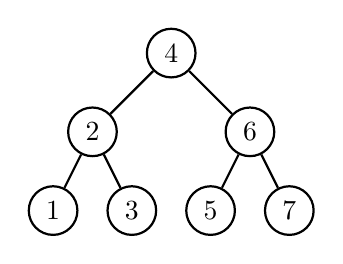
\begin{tikzpicture}[thick, 
	level 1/.style={sibling distance=2cm},
	level 2/.style={sibling distance=1cm},
	level 3/.style={sibling distance=0.5cm},
	level distance = 1cm
	]
\node [circle,draw] (n4){$4$}
  child {node [circle,draw] (n2) {$2$}
  	child {node [circle,draw] (n1) {$1$}}
  	child {node [circle,draw] (n3) {$3$}}
  }
  child {node [circle,draw] (n6) {$6$}
  	child {node [circle,draw] (n5) {$5$}}
  	child {node [circle,draw] (n7) {$7$}}
 };
%\tikzstyle{nodo}=[shape=circle,draw,thick,inner sep=0pt,minimum size=25pt,draw=black]
%\node [nodo] (n4) {$4$};
%\node [nodo] (n2) [below of=n4] {$2$};
%\node [nodo] (n6) [below of=n4] {$6$};
%\path (n4) edge [thick] (n2);
%\path (n4) edge [thick] (n6);
%\node [mode] (m1) [right of=t2] {{\large\bf R}};
%\path (m1) edge [thick] (t1);
%\node [task] (t5) [below of=t4] {{\large$t_5$}};
%\node [mode] (m3) [right of=t5] {{\large\bf RW}}
%edge [thick] (t5)
%edge [<-,thick] (m2);
\end{tikzpicture}
\caption{Exemplo de árvore de busca binária.}
\label{aula05:fig:arv}
\end{figure}

Os passos na operação de {\bf busca} para uma chave $x$ são:
\begin{enumerate}
\item Compare com a chave que está na raiz.
\item Se $x$ é menor, vá para a sub-árvore esquerda.
\item Se $x$ é maior, vá para a sub-árvore direita.
\item Repita o processo recursivamente, até que a chave procurada seja
encontrada ou um nó folha é atingido.
\end{enumerate}
O algoritmo de busca em árvore binária é ilustrado na figura~\ref{aula05:algo:arv:busca}.
\begin{figure}[!htb]
\centering
\begin{framed}
\begin{lstlisting}
Arv* ArvBusca( Arv* a, int chave ) {
	if( a == NULL )        return NULL;
	if( a.chave == chave)  return a;
	if( chave < a.chave )  return ArvBusca( a->esq, chave );
	else                   return ArvBusca( a->dir, chave );
	return NULL;
}
\end{lstlisting}
\end{framed}
\caption{Algoritmo de busca em árvore binária.}
\label{aula05:algo:arv:busca}
\end{figure}

O procedimento de {\bf inserção} é:
\begin{enumerate}
\item Executar o procedimento de busca da chave a ser inserida.
\item O ponto onde deveria estar a chave é o ponto de inserção.
\end{enumerate}

O procedimento de {\bf remoção} não é tão simples:
\begin{enumerate}
\item Executar o procedimento de busca da chave a ser removida.
\item Se o nó contém o registro a ser removido possui no máximo
um descendente, trocar o nó a ser removido pelo seu descendente.
\item Se possuir dois descendentes o registro a ser removido deve ser primeiro
substituído:
	\begin{itemize}
	\item pelo registro mais à direita na sub-árvore esquerda.
	\item ou pelo registro mais à esquerda na sub-árvore direita.
	\end{itemize}
\end{enumerate}

{\bf Análise} -- o número de comparações em uma busca com sucesso no melhor caso é 
$C(n)= 1$, pior caso $C(n) = n$ e caso médio $C(n) = \log  n$.
O pior caso ocorre quando as chaves são inseridas em ordem crescente ou decrescente.

%%%%%%%%%%%%%%%%%%%%%%%%%%%%%%%%%%%%%%%%%%%%%%%%%%%%%%%%%%%%%%%%%%%%%%%%%%%%%%%
\section{Propriedades em árvores}
%%%%%%%%%%%%%%%%%%%%%%%%%%%%%%%%%%%%%%%%%%%%%%%%%%%%%%%%%%%%%%%%%%%%%%%%%%%%%%%

%%%%%%%%%%%%%%%%%%%%%%%%%%%%%%%%%%%%%%%%%%%%%%%%%%%%%%%%%%%%%%%%%%%%%%%%%%%%%%%
\subsection{Percurso em árvores}

Há três tipos de percurso em árvores:
\begin{description}
\item[Pré-ordem -] o nó é visitado antes das sub-árvores descendentes. 
\item[Pós-ordem -] o nó é visitado depois das sub-árvores descendentes.
\item[Em-ordem -] em árvores binárias, o nó é visitado depois da sub-árvore
da esquerda e antes da sub-árvore da direita.
\end{description}

%%%%%%%%%%%%%%%%%%%%%%%%%%%%%%%%%%%%%%%%%%%%%%%%%%%%%%%%%%%%%%%%%%%%%%%%%%%%%%%
\subsection{Propriedades em árvores binárias}

Dada a notação:
\begin{itemize}
\item $n$ - número de nós.
\item $e$ - número de nós externos (folhas).
\item $i$ - número de nós internos (não folhas).
\item $h$ - altura.
\end{itemize}
Segue as seguintes propriedades sobre árvores binárias:
\begin{itemize}
\item $e = i + 1$.
\item $n = 2e - 1$.
\item $h \leq i$.
\item $h \leq (n-1)/2$.
\item $e \leq 2^h$.
\item $h \geq \log e$.
\item $ \geq \log (n+1) -1$.
\end{itemize}



%%%%%%%%%%%%%%%%%%%%%%%%%%%%%%%%%%%%%%%%%%%%%%%%%%%%%%%%%%%%%%%%%%%%%%%%%%%%%%%
\section{Árvores de busca balanceadas}
%%%%%%%%%%%%%%%%%%%%%%%%%%%%%%%%%%%%%%%%%%%%%%%%%%%%%%%%%%%%%%%%%%%%%%%%%%%%%%%

Uma limitação das árvores binárias de pesquisa é a ordem em que os elementos
são inseridos. Por exemplo, as ordens de inserção abaixo:
\begin{itemize}
\item ordem $1, 2, 3, 4, 5, 6, 7$ gera uma {\bf árvore degenerada} (todo nó
tem apenas um filho).
\item ordem $4, 6, 2, 5, 1, 7, 3$ gera uma árvore binária completa.
\end{itemize}
O que afeta diretamente o desempenho na busca de elementos.

Idealmente deseja-se que a árvore esteja {\bf completamente balanceada}.
A distância média para qualquer nó da árvore é mínima.
No entanto, manter uma árvore completamente balanceada tem alto custo.
Uma solução é procurar uma solução intermediária que possa manter a árvore
balanceada.

Uma {\bf árvore de busca balanceada} garante uma altura de $O(\log n)$
quando implementa um conjunto dinâmico de $n$ itens.
Alguns exemplos de árvores balanceadas são AVL, árvores 2-3, árvores 2-3-4,
B-trees e árvore rubro-negra.

%%%%%%%%%%%%%%%%%%%%%%%%%%%%%%%%%%%%%%%%%%%%%%%%%%%%%%%%%%%%%%%%%%%%%%%%%%%%%%%
\subsection{Árvore AVL}

Uma árvore binária é denominada {\bf AVL} (dos seus criadores Georgy
Adelson-Velsky e Landis) se para todos os nós, {\bf as alturas de suas duas
sub-árvores diferem no máximo em uma unidade}, sendo assim balanceada.
Operações de consulta, inserção e remoção de nós tem custo $O(\log n)$.

O {\bf fator de balanceamento} (FB) de um nó é a diferença entre
a altura da sub-árvore da esquerda e a altura da sub-árvore da direita.
Se não existir uma sub-árvore, a altura é zero.
Os resultados de um FB são:
\begin{itemize}
\item $> 0$ - sub-árvore da direita é menor.
\item $< 0$ - sub-árvore da esquerda é menor.
\item $= 0$ - sub-árvores tem a mesma altura.
\end{itemize}
Os valores válidos de FB são $-1$ (sub-árvore da esquerda é menor), $0$, $1$
(sub-árvore da direita é menor).

\subsubsection{Inserção}

O nó é inserido como em uma árvore binária comum.
Se a inserção não degenerar a árvore, o processo termina.
Caso contrário, é necessário:
\begin{enumerate}
\item encontrar o nó cujo FB esteja fora do intervalo (pivô).
\item realizar uma rotação na árvore a partir do nó ``pivô''
(rotação simples ou rotação dupla).
\end{enumerate}
Apenas uma rotação (simples ou dupla) é necessária.
Após essa rotação, a árvore já estará balanceada.
Há quatro possibilidades de rotação:
\begin{itemize}
\item 2 casos externos (direita e esquerda) com rotação simples.
\item 2 casos internos (direta e esquerda) com rotação dupla.
\end{itemize}

\subsubsection{Rotação}

Suponha que $\alpha$ seja um pivô, nos casos externos, uma rotação simples é necessária 
caso a inserção ocorra na \textbf{sub-árvore à esquerda do filho à esquerda de} $\alpha$
ou na \textbf{sub-árvore à direita do filho à direita de} $\alpha$.
A figura~\ref{aula05:avl:rot:simples1} demonstra dois exemplos de rotação
simples a direta.
%
\begin{figure}[!htb]
\centering
  \begin{minipage}{0.2\textwidth}
	\centering
	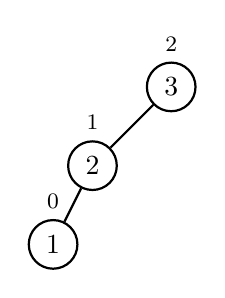
\begin{tikzpicture}[thick, 
		level 1/.style={sibling distance=2cm},
		level 2/.style={sibling distance=1cm},
		level 3/.style={sibling distance=1cm},
		level distance = 1cm
		]
	\node [circle,draw,label=above:{\footnotesize 2}] (n3) {3}
	  child {
		node [circle,draw,label=above:{\footnotesize 1}] (n2) {2}
			child { node [circle,draw,label=above:{\footnotesize 0}] (n1) {1} }
			child[missing] {}
	  }
	  child[missing] {};
	\end{tikzpicture}
  \end{minipage}
%
  \begin{minipage}{0.2\textwidth}
	\centering
	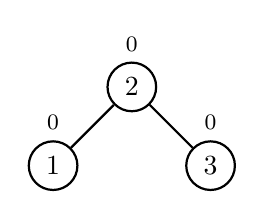
\begin{tikzpicture}[thick, 
		level 1/.style={sibling distance=2cm},
		level 2/.style={sibling distance=1cm},
		level 3/.style={sibling distance=1cm},
		level distance = 1cm
		]
	\node [circle,draw,label=above:{\footnotesize 0}] (n2) {2}
		child { node [circle,draw,label=above:{\footnotesize 0}] (n1) {1} }
		child { node [circle,draw,label=above:{\footnotesize 0}] (n3) {3} };
	\end{tikzpicture}
  \end{minipage}
  %
  \vline
  %
  \begin{minipage}{0.25\textwidth}
	\centering
	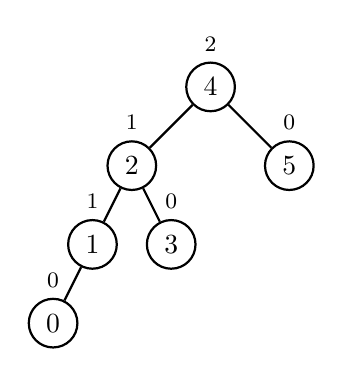
\begin{tikzpicture}[thick,
		level 1/.style={sibling distance=2cm},
		level 2/.style={sibling distance=1cm},
		level 3/.style={sibling distance=1cm},
		level distance = 1cm ]
	\node [circle,draw,label=above:{\footnotesize 2}] (n4) {4}
	  child {
		node [circle,draw,label=above:{\footnotesize 1}] (n2) {2}
		child {
			node [circle,draw,label=above:{\footnotesize 1}] (n1) {1}
			child { node[circle,draw,label=above:{\footnotesize 0}] (n0) {0} }
			child[missing] {}
		}
		child { node[circle,draw,label=above:{\footnotesize 0}] (n3) {3} }
	  }
	  child { node [circle,draw,label=above:{\footnotesize 0}] (n5) {5} };
	\end{tikzpicture}
  \end{minipage}
%
  \begin{minipage}{0.2\textwidth}
	\centering
	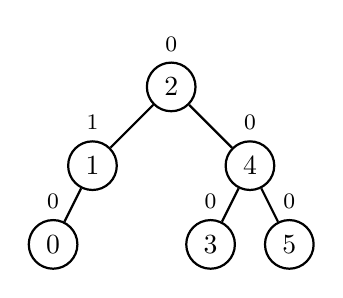
\begin{tikzpicture}[thick,
		level 1/.style={sibling distance=2cm},
		level 2/.style={sibling distance=1cm},
		level 3/.style={sibling distance=1cm},
		level distance = 1cm ]
	\node [circle,draw,label=above:{\footnotesize 0}] (n2) {2}
	  child {
		node [circle,draw,label=above:{\footnotesize 1}] (n1) {1}
		child { node [circle,draw,label=above:{\footnotesize 0}] (n0) {0} }
		child[missing] {}
	  }
	 child {
		 node[circle,draw,label=above:{\footnotesize 0}] (n4) {4}
		child { node [circle,draw,label=above:{\footnotesize 0}] (n3) {3} }
		child { node [circle,draw,label=above:{\footnotesize 0}] (n5) {5} }
	 };
	\end{tikzpicture}
  \end{minipage}
\caption{Dois exemplos de AVL com rotação simples para a direita e cada nó com seu FB.}
\label{aula05:avl:rot:simples1}
\end{figure}

Nos casos internos, suponha que o pivô seja $\alpha$, 
uma rotação dupla é necessária caso a inserção ocorra 
na {\bf sub-árvore à esquerda do filho à direita de} $\alpha$ ou
na {\bf sub-árvore à direita do filho à esquerda de} $\alpha$.
Uma rotação dupla equivale a duas rotações simples em sequência.
A figura~\ref{aula05:avl:rot:dupla1} demonstra um exemplo de rotação
dupla a direta.
%
\begin{figure}[!htb]
\centering
  \begin{minipage}{0.3\textwidth}
	\centering
	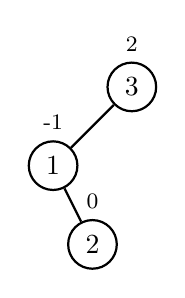
\begin{tikzpicture}[thick, 
		level 1/.style={sibling distance=2cm},
		level 2/.style={sibling distance=1cm},
		level 3/.style={sibling distance=1cm},
		level distance = 1cm
		]
	\node [circle,draw,label=above:{\footnotesize 2}] (n3) {3}
	  child {
		node [circle,draw,label=above:{\footnotesize -1}] (n1) {1}
			child[missing] {}
			child { node [circle,draw,label=above:{\footnotesize 0}] (n2) {2} }
	  }
	  child[missing] {};
	\end{tikzpicture}
  \end{minipage}
%
  \vline
%
  \begin{minipage}{0.3\textwidth}
	\centering
	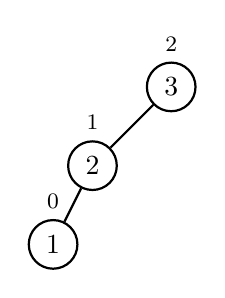
\begin{tikzpicture}[thick, 
		level 1/.style={sibling distance=2cm},
		level 2/.style={sibling distance=1cm},
		level 3/.style={sibling distance=1cm},
		level distance = 1cm
		]
	\node [circle,draw,label=above:{\footnotesize 2}] (n3) {3}
	  child {
		node [circle,draw,label=above:{\footnotesize 1}] (n2) {2}
			child { node [circle,draw,label=above:{\footnotesize 0}] (n1) {1} }
			child[missing] {}
	  }
	  child[missing] {};
	\end{tikzpicture}
  \end{minipage}
%
  \vline
%
  \begin{minipage}{0.3\textwidth}
	\centering
	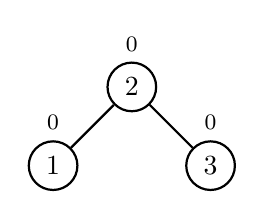
\begin{tikzpicture}[thick, 
		level 1/.style={sibling distance=2cm},
		level 2/.style={sibling distance=1cm},
		level 3/.style={sibling distance=1cm},
		level distance = 1cm
		]
	\node [circle,draw,label=above:{\footnotesize 0}] (n2) {2}
		child { node [circle,draw,label=above:{\footnotesize 0}] (n1) {1} }
		child { node [circle,draw,label=above:{\footnotesize 0}] (n3) {3} };
	\end{tikzpicture}
  \end{minipage}
\caption{Exemplo de AVL com rotação dupla, e cada nó com seu FB.}
\label{aula05:avl:rot:dupla1}
\end{figure}

\subsubsection{Remoção}

A remoção em AVL é similar a inserções, mas mais complexas.
Incialmente, usa-se a estratégia de remoção das árvores não balanceadas.
Porém, pode gerar desequilíbrio e exigir balanceamento.
Rotações simples e duplas são necessárias durante esse balanceamento.

Após o balanceamento, pode haver desequilíbrio em níveis superiores.
Assim, deve-ser analisar também esses níveis superiores.
A figura~\ref{aula05:avl:rm:ex1} demonstra um exemplo de remoção
com rotação simples a esquerda.
%
\begin{figure}[!htb]
\centering
  \begin{minipage}{0.3\textwidth}
	\centering
	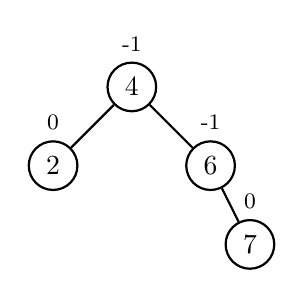
\begin{tikzpicture}[thick, 
		level 1/.style={sibling distance=2cm},
		level 2/.style={sibling distance=1cm},
		level 3/.style={sibling distance=1cm},
		level distance = 1cm
		]
	\node [circle,draw,label=above:{\footnotesize -1}] (n4) {4}
	  child { node [circle,draw,label=above:{\footnotesize 0}] (n2) {2} }
	  child {
		node [circle,draw,label=above:{\footnotesize -1}] (n6) {6}
			child[missing] {}
			child { node [circle,draw,label=above:{\footnotesize 0}] (n7) {7} }
	  };
	\end{tikzpicture}
  \end{minipage}
%
  \vline
%
  \begin{minipage}{0.3\textwidth}
	\centering
	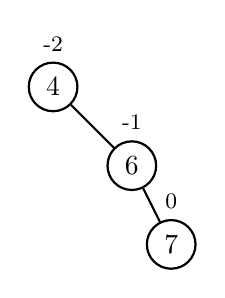
\begin{tikzpicture}[thick, 
		level 1/.style={sibling distance=2cm},
		level 2/.style={sibling distance=1cm},
		level 3/.style={sibling distance=1cm},
		level distance = 1cm
		]
	\node [circle,draw,label=above:{\footnotesize -2}] (n4) {4}
	  child[missing] {}
	  child {
		node [circle,draw,label=above:{\footnotesize -1}] (n6) {6}
			child[missing] {}
			child { node [circle,draw,label=above:{\footnotesize 0}] (n7) {7} }
	  };
	\end{tikzpicture}
  \end{minipage}
%
  \vline
%
  \begin{minipage}{0.3\textwidth}
	\centering
	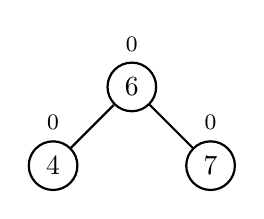
\begin{tikzpicture}[thick, 
		level 1/.style={sibling distance=2cm},
		level 2/.style={sibling distance=1cm},
		level 3/.style={sibling distance=1cm},
		level distance = 1cm
		]
	\node [circle,draw,label=above:{\footnotesize 0}] (n6) {6}
		child { node [circle,draw,label=above:{\footnotesize 0}] (n4) {4} }
		child { node [circle,draw,label=above:{\footnotesize 0}] (n7) {7} };
	\end{tikzpicture}
  \end{minipage}
\caption{Exemplo de remoção em AVL (nó 2) com rotação simples a esquerda.}
\label{aula05:avl:rm:ex1}
\end{figure}

\subsubsection{Análise}

Entre as possíveis operações temos:
\begin{itemize}
\item {\bf rotação} única custo $O(1)$ pois é constante.
\item {\bf busca}  é $O(\log n)$ pois a altura de árvore é $O(\log n)$
e não necessita balanceamento.
\item {\bf inserção} é $O(\log n)$ com o custo da busca incial de $O(\log n)$
e mais balanceamento para manter FP tem custo $O(\log n)$.
\item {\bf remoção} é $O(\log n)$ com a busca inicial de $O(\log n)$ mais
balanceamento para manter FP tem custo $O(\log n)$.
\end{itemize}

%%%%%%%%%%%%%%%%%%%%%%%%%%%%%%%%%%%%%%%%%%%%%%%%%%%%%%%%%%%%%%%%%%%%%%%%%%%%%%%
\subsection{Árvore rubro-negra}

Uma  árvore rubro-negra (\emph{red-black tree}) é um tipo de árvore de pesquisa
binária com uma propriedade adicional (1 bit) que representa a \textbf{cor} de
um nó.
Além disso, as folhas não armazenam dados sendo denotados por \textsc{NIL}
(nulo).
A figura~\ref{aula05:redblack:ex1} demonstra um exemplo de árvore rubro-negra.
%
\begin{figure}[!htb]
\centering
  \begin{minipage}{\textwidth}
	\centering
	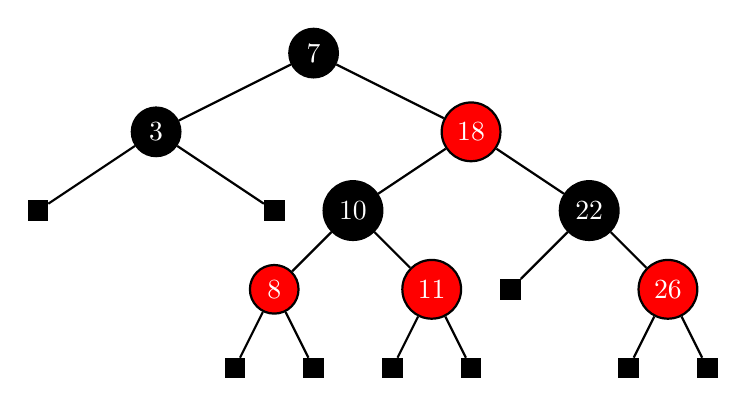
\begin{tikzpicture}[thick, 
		level 1/.style={sibling distance=4cm},
		level 2/.style={sibling distance=3cm},
		level 3/.style={sibling distance=2cm},
		level 4/.style={sibling distance=1cm},
		level distance = 1cm
		]
	\node [circle,draw,white,fill=black,draw=black] (n7) {7}
	  child {
		  node [circle,draw,white,fill=black,draw=black] (n3) {3}
		  child { node [rectangle,draw,white,fill=black,draw=black,minimum size=0.5em] {} }
		  child { node [rectangle,draw,white,fill=black,draw=black,minimum size=0.5em] {} }
	  }
	  child {
		node [circle,draw,white,fill=red,draw=black] (n18) {18}
		child {
		  node [circle,draw,white,fill=black,draw=black] (n10) {10}
		  child {
			node [circle,draw,white,fill=red,draw=black] (n8) {8}
			  child { node [rectangle,draw,white,fill=black,draw=black,minimum size=0.5em] {} }
			  child { node [rectangle,draw,white,fill=black,draw=black,minimum size=0.5em] {} }
		  }
		  child {
			node [circle,draw,white,fill=red,draw=black] (n11) {11}
			  child { node [rectangle,draw,white,fill=black,draw=black,minimum size=0.5em] {} }
			  child { node [rectangle,draw,white,fill=black,draw=black,minimum size=0.5em] {} }
		  }
		}
		child {
		  node [circle,draw,white,fill=black,draw=black] (n22) {22}
			  child { node [rectangle,draw,white,fill=black,draw=black,minimum size=0.5em] {} }
			  child {
				node [circle,draw,white,fill=red,draw=black] (n26) {26}
				  child { node [rectangle,draw,white,fill=black,draw=black,minimum size=0.5em] {} }
				  child { node [rectangle,draw,white,fill=black,draw=black,minimum size=0.5em] {} }
			  }
		}
	  };
	\end{tikzpicture}
  \end{minipage}
\caption{Exemplo de árvore rubro-negra.}
\label{aula05:redblack:ex1}
\end{figure}

As propriedades de uma rubro-negra são:
\begin{enumerate}
\item Cada nó é vermelho ou preto.
\item A raiz e todas as folhas (\textsc{NIL}) são preto.
\item Se um nós é vermelho, então seu antecessor (nó pai) é preto.
\item Todos os caminhos simples de qualquer nó $x$ para uma folha descendente 
tem o mesmo número de nós pretos.
\end{enumerate}

\begin{theorem}
Uma árvore rubro-negra com $n$ elementos tem altura
\[ h \leq 2 \log (n + 1) \].
\end{theorem}

\subsubsection{Rotações}

Inserções e remoções custam $O(\log n)$ e, como podem modificar a árvore,
o resultado pode violar as propriedades de uma rubro-negra.
A rotação muda cores de nós e a estrutura da árvore.
Há dois tipos de rotação em árvores rubro-negras: rotações a esquerda e 
rotações a direita.
As rotação são explicadas na inserção.

\subsubsection{Inserção}

A inserção adiciona um nó $x$ de cor vermelha na árvore da mesma forma que 
em uma árvore binária de busca.
Nesse caso, apenas a propriedade 3 de rubro-negras pode ser violada.
Caso a propriedade 3 foi violada, mover para o nó pai por recoloração até que
as propriedades sejam respeitadas através de rotações e recolorações.

Os passos da inserção envolvem 3 casos. Nos exemplos abaixo,
cada quadrado azul representa uma sub-árvore com uma raiz preta, e todas
tem a mesma altura em nós preto.
\begin{enumerate}
\item insere na árvore o nó $x$ com cor vermelha.
\item se propriedade 3 foi violada:
	\begin{enumerate}
	\item {\bf Caso 1} - ocorre quando o nó pai de $x$ e $z$ são vermelhos
	(figura~\ref{aula05:redblack:ex2}).
	Consiste em recolorir o nó pai de $x$ e tios (nós vizinhos do pai de $x$, ou
	filhos do avô de $x$).
	O novo $x$ será o nó avô do antigo $x$ .
	\item {\bf Caso 2} - quando o pai de $x$ é vermelho e $z$ é preto
		(figura~\ref{aula05:redblack:ex3}).
		É feita uma rotação para esquerda, e automaticamente cai no {\bf Caso 3}.
	\item {\bf Caso 3} - novamente quando o pai de $x$ é vermelho e $z$ é preto
		(figura~\ref{aula05:redblack:ex4}).
		É feita uma rotação para direita, ainda recolorir pai de $x$ e avô de $x$.
	\end{enumerate}
\end{enumerate}

\begin{figure}[!htb]
\centering
  \begin{minipage}{0.4\textwidth}
	\centering
	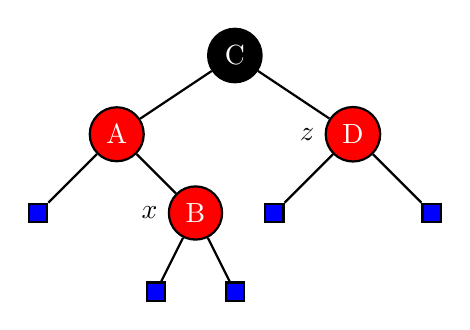
\begin{tikzpicture}[thick, 
		level 1/.style={sibling distance=3cm},
		level 2/.style={sibling distance=2cm},
		level 3/.style={sibling distance=1cm},
		level 4/.style={sibling distance=0.5cm},
		level distance = 1cm
		]
	\node [circle,draw,white,fill=black,draw=black] (c) {C}
	  child {
		  node [circle,draw,white,fill=red,draw=black] (a) {A}
		  child { node [rectangle,draw,white,fill=blue,draw=black] {} }
		  child {
			  node [circle,draw,white,fill=red,draw=black,label=left:$x$] (b) {B} 
			  child { node [rectangle,draw,white,fill=blue,draw=black] {} }
			  child { node [rectangle,draw,white,fill=blue,draw=black] {} }
		  }
	  }
	  child {
		  node [circle,draw,white,fill=red,draw=black,label=left:$z$] (d) {D}
		  child { node [rectangle,draw,white,fill=blue,draw=black] {} }
		  child { node [rectangle,draw,white,fill=blue,draw=black] {} }
	  };
	\end{tikzpicture}
  \end{minipage}
  %
  \vline
  %
  \begin{minipage}{0.4\textwidth}
	\centering
	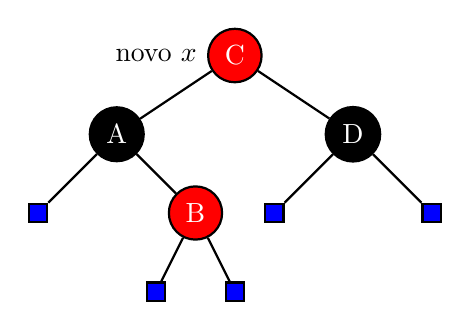
\begin{tikzpicture}[thick, 
		level 1/.style={sibling distance=3cm},
		level 2/.style={sibling distance=2cm},
		level 3/.style={sibling distance=1cm},
		level 4/.style={sibling distance=0.5cm},
		level distance = 1cm
		]
	\node [circle,draw,white,fill=red,draw=black,label=left:novo $x$] (c) {C}
	  child {
		  node [circle,draw,white,fill=black,draw=black] (a) {A}
		  child { node [rectangle,draw,white,fill=blue,draw=black] {} }
		  child {
			  node [circle,draw,white,fill=red,draw=black] (b) {B}
			  child { node [rectangle,draw,white,fill=blue,draw=black] {} }
			  child { node [rectangle,draw,white,fill=blue,draw=black] {} }
		  }
	  }
	  child {
		  node [circle,draw,white,fill=black,draw=black] (d) {D}
		  child { node [rectangle,draw,white,fill=blue,draw=black] {} }
		  child { node [rectangle,draw,white,fill=blue,draw=black] {} }
	  };
	\end{tikzpicture}
  \end{minipage}
\caption{Caso 1 da inserção em árvore rubro-negra: recoloração}
\label{aula05:redblack:ex2}
\end{figure}

\begin{figure}[!htb]
\centering
  \begin{minipage}{0.4\textwidth}
	\centering
	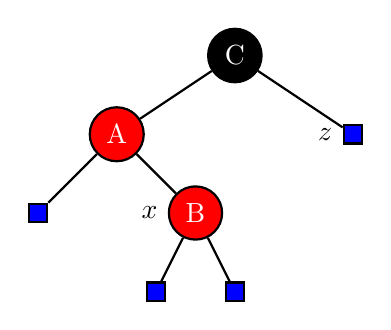
\begin{tikzpicture}[thick, 
		level 1/.style={sibling distance=3cm},
		level 2/.style={sibling distance=2cm},
		level 3/.style={sibling distance=1cm},
		level 4/.style={sibling distance=0.5cm},
		level distance = 1cm
		]
	\node [circle,draw,white,fill=black,draw=black] (c) {C}
	  child {
		  node [circle,draw,white,fill=red,draw=black] (a) {A}
		  child { node [rectangle,draw,white,fill=blue,draw=black] {} }
		  child {
			  node [circle,draw,white,fill=red,draw=black,label=left:$x$] (b) {B}
			  child { node [rectangle,draw,white,fill=blue,draw=black] {} }
			  child { node [rectangle,draw,white,fill=blue,draw=black] {} }
		  }
	  }
	  child { node [rectangle,draw,white,fill=blue,draw=black,label=left:$z$] {} };
	\end{tikzpicture}
  \end{minipage}
  %
  \vline
  %
  \begin{minipage}{0.4\textwidth}
	\centering
	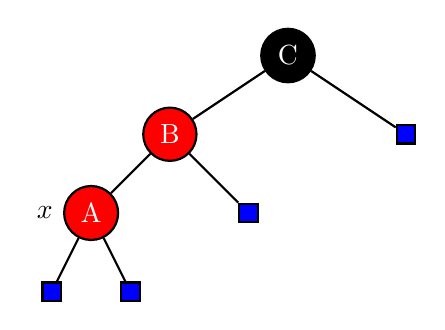
\begin{tikzpicture}[thick, 
		level 1/.style={sibling distance=3cm},
		level 2/.style={sibling distance=2cm},
		level 3/.style={sibling distance=1cm},
		level 4/.style={sibling distance=0.5cm},
		level distance = 1cm
		]
	\node [circle,draw,white,fill=black,draw=black] (c) {C}
	  child {
		  node [circle,draw,white,fill=red,draw=black] (b) {B}
		  child {
			  node [circle,draw,white,fill=red,draw=black,label=left:$x$] (a) {A}
			  child { node [rectangle,draw,white,fill=blue,draw=black] {} }
			  child { node [rectangle,draw,white,fill=blue,draw=black] {} }
		  }
		  child { node [rectangle,draw,white,fill=blue,draw=black] {} }
	  }
	  child { node [rectangle,draw,white,fill=blue,draw=black] {} };
	\end{tikzpicture}
  \end{minipage}
\caption{Caso 2 da inserção em árvore rubro-negra: rotação para esquerda.}
\label{aula05:redblack:ex3}
\end{figure}

\begin{figure}[!htb]
\centering
  \begin{minipage}{0.4\textwidth}
	\centering
	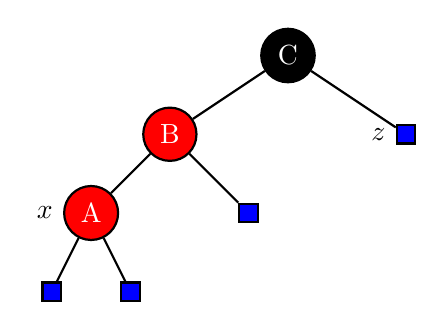
\begin{tikzpicture}[thick, 
		level 1/.style={sibling distance=3cm},
		level 2/.style={sibling distance=2cm},
		level 3/.style={sibling distance=1cm},
		level 4/.style={sibling distance=0.5cm},
		level distance = 1cm
		]
	\node [circle,draw,white,fill=black,draw=black] (c) {C}
	  child {
		  node [circle,draw,white,fill=red,draw=black] (b) {B}
		  child {
			  node [circle,draw,white,fill=red,draw=black,label=left:$x$] (a) {A}
			  child { node [rectangle,draw,white,fill=blue,draw=black] {} }
			  child { node [rectangle,draw,white,fill=blue,draw=black] {} }
		  }
		  child { node [rectangle,draw,white,fill=blue,draw=black] {} }
	  }
	  child { node [rectangle,draw,white,fill=blue,draw=black,label=left:$z$] {} };
	\end{tikzpicture}
  \end{minipage}
  %
  \vline
  %
  \begin{minipage}{0.4\textwidth}
	\centering
	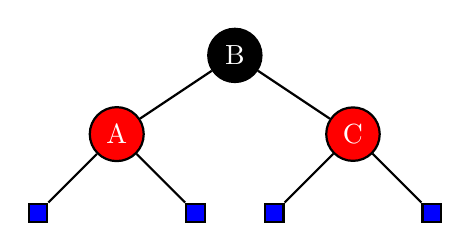
\begin{tikzpicture}[thick, 
		level 1/.style={sibling distance=3cm},
		level 2/.style={sibling distance=2cm},
		level 3/.style={sibling distance=1cm},
		level 4/.style={sibling distance=0.5cm},
		level distance = 1cm
		]
	\node [circle,draw,white,fill=black,draw=black] (b) {B}
	  child {
		  node [circle,draw,white,fill=red,draw=black] (a) {A}
		  child { node [rectangle,draw,white,fill=blue,draw=black] {} }
		  child { node [rectangle,draw,white,fill=blue,draw=black] {} }
	  }
	  child { 
		  node [circle,draw,white,fill=red,draw=black] (c) {C}
		  child { node [rectangle,draw,white,fill=blue,draw=black] {} }
		  child { node [rectangle,draw,white,fill=blue,draw=black] {} }
	};
	\end{tikzpicture}
  \end{minipage}
\caption{Caso 3 da inserção em árvore rubro-negra: rotação para direita.}
\label{aula05:redblack:ex4}
\end{figure}

%\subsubsection{Remoção}

\subsubsection{Análise}

Como a altura de uma rubro-negra de $n$ nós é $O(\log n)$, o custo da inserção
é $O(\log n)$.
Esse custo inclui o custo de inserção $O(\log n)$, como em uma árvore binária
de busca, e rotações para manter a árvore de no máximo $O(\log n)$.
Não obstante, ele não executa mais do que 2 rotações porque sempre executa 
o caso 1 e em seguida caso 2 ou caso 3.

%%%%%%%%%%%%%%%%%%%%%%%%%%%%%%%%%%%%%%%%%%%%%%%%%%%%%%%%%%%%%%%%%%%%%%%%%%%%%%%%
%\subsection{Árvore SBB}
%
%\todo[inline]{Prox. aula.}

%%%%%%%%%%%%%%%%%%%%%%%%%%%%%%%%%%%%%%%%%%%%%%%%%%%%%%%%%%%%%%%%%%%%%%%%%%%%%%%
\section{Tabelas \textsc{Hash}}
%%%%%%%%%%%%%%%%%%%%%%%%%%%%%%%%%%%%%%%%%%%%%%%%%%%%%%%%%%%%%%%%%%%%%%%%%%%%%%%

Em uma tabela \textsc{hash} os registros armazenados em uma tabela são
diretamente endereçados a partir de uma transformação aritmética sobre a chave
de pesquisa.
A operação é chamada transformação de chave ou \emph{hashing}.

A pesquisa com transformação de chave é composta de duas etapas:
\begin{enumerate}
\item Computar o valor a {\bf função de transformação}, que 
transforma a chave de pesquisa em um endereço da tabela.

\item Considerando que duas ou mais chaves podem ser transformadas em um
mesmo endereço de tabela, é necessário existir um método lidar
com \textbf{colisões}.
\end{enumerate}

Algumas {\bf colisões} irão ocorrer qualquer que seja a função de transformação,
e tais colisões têm de ser resolvidas.
Mesmo com alguma função de transformação que distribua registros de forma uniforme,
existe uma alta probabilidade de haver colisões.

%%%%%%%%%%%%%%%%%%%%%%%%%%%%%%%%%%%%%%%%%%%%%%%%%%%%%%%%%%%%%%%%%%%%%%%%%%%%%%%%
\subsection{Funções de hash}

Uma função de hash $h$ mapea um universo $U$  de todas as chaves em 
\emph{slots} de uma tabela hash $T[0..m-1]$ para $S$ sendo
$S = \{0, 1, ..., m-1\}$ onde $m$ é muito menor que o universo $U$.
O valor da chave $h(k)$ é o {\bf valor hash} da chave $k$.
A função hash reduz o intervalo de índices e tamanho de um vetor.
Ao invés de $|U|$, o vetor (tabela $T$) tem tamanho $m$ sendo $|U| > m$.

Um método simples de \emph{hashing} é o resto da divisão por $m$
\begin{equation*}
h(k) = k\; mod\; m
\end{equation*}
onde $k$ é a chave como um inteiro.

{\bf Cuidado} na escolha do valor de $m$. $m$ deve ser um número primo não muito
próximo do exponencial de $2$ ou $10$ e não usado com frequência.

Existem diversos métodos para armazenar $n$ registros em uma tabela de tamanho
$m > n$ em que utilizam lugares vázios na própria tabela para resolver
colisões.

%%%%%%%%%%%%%%%%%%%%%%%%%%%%%%%%%%%%%%%%%%%%%%%%%%%%%%%%%%%%%%%%%%%%%%%%%%%%%%%%
\subsection{Encadeamento}

No caso de colisões, uma solução simples é construir uma lista 
encadeada para cada endereço da tabela.
Dessa forma, todas as chaves com o mesmo endereço são encadeadas em uma lista.
O {\bf fator de balanceamento} de $T$ é $\alpha = n/m$ onde $n$ é o número
de chaves na tabela e $m$ o tamanho da tabela.
A figura~\ref{aula05:fig:hash} ilustra um exemplo de tabela hash com alguns
slots com colisões.
%
\begin{figure}[ht]
\centering
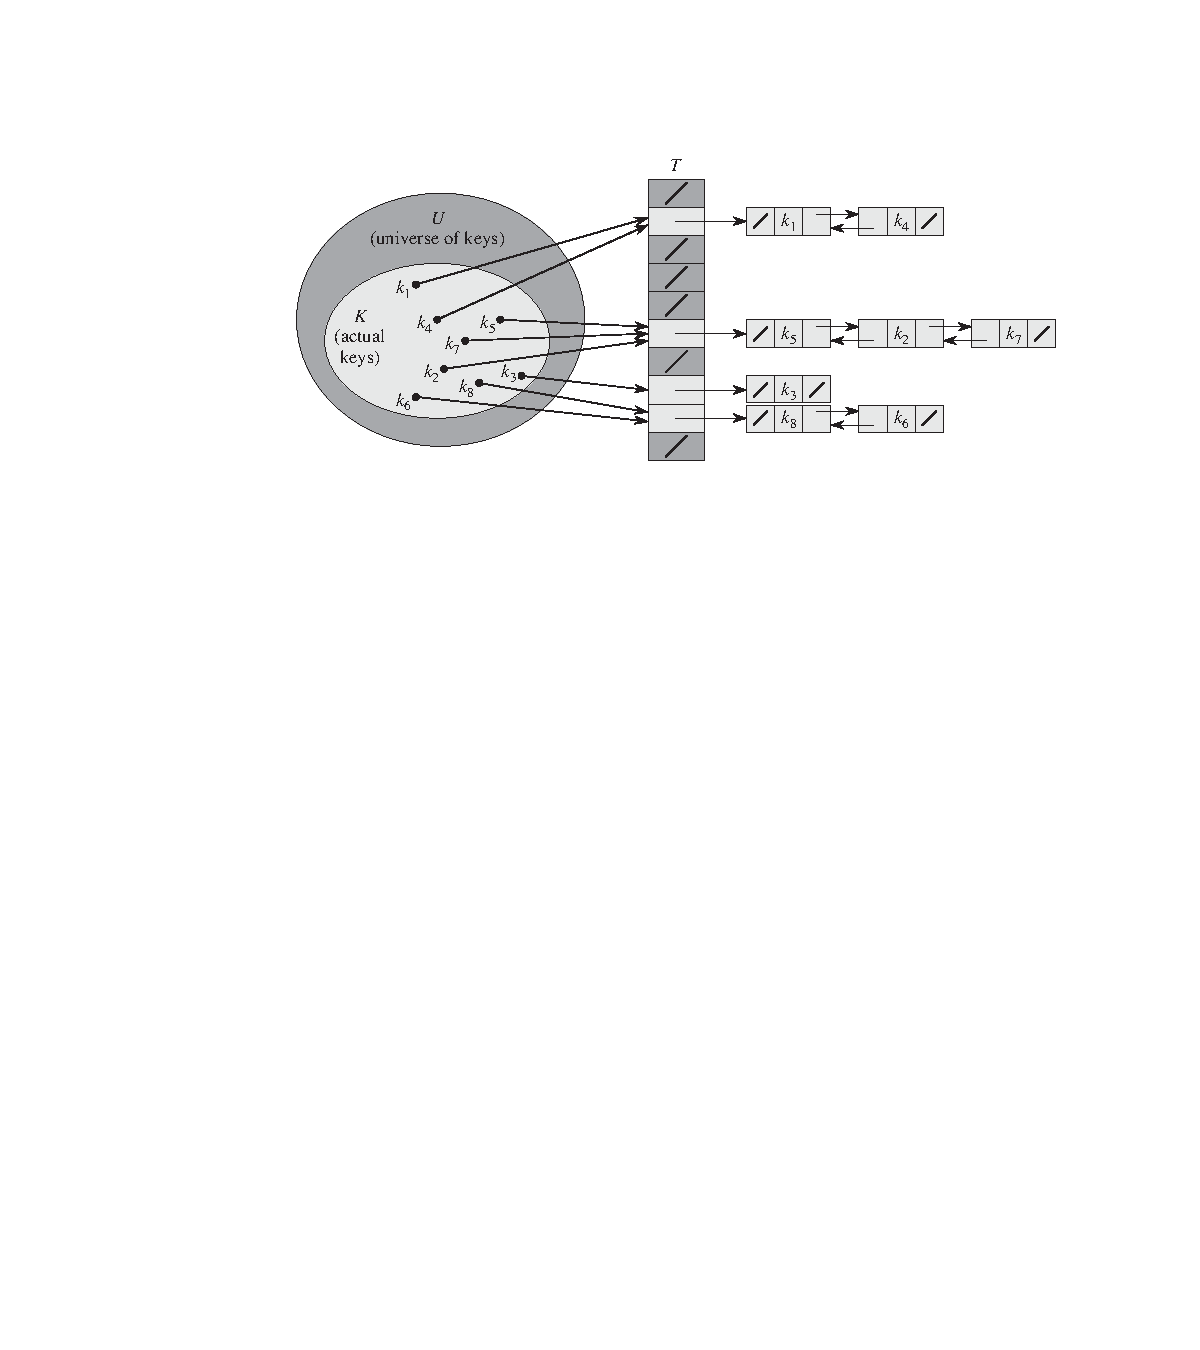
\includegraphics[width=0.8\textwidth]{aula05-hash1}
\caption{Exemplo de uma tabela hash com colisões.}
\label{aula05:fig:hash}
\end{figure}

O custo de busca para uma chave é $O(1 + \alpha)$ onde custo $1$ é aplicar
a função hash e acessar o slot, e $\alpha$ a busca na lista.
Então, o custo é $O(1)$ se $\alpha = O(1)$.

%%%%%%%%%%%%%%%%%%%%%%%%%%%%%%%%%%%%%%%%%%%%%%%%%%%%%%%%%%%%%%%%%%%%%%%%%%%%%%%%
\subsection{Endereçamento aberto}

No {\bf endereçamento aberto} todas as chaves são armazenadas na própria 
tabela, sem uso de memória adicional.
Se o endereço $e$ estiver ocupado tenta no endereço $e+1, e+2, ... n, 1, 2, ...  e-1$.

% TODO exemplo ziviane pg 86
Entre as várias propostas, a mais simples é \emph{hashing linear} dada por
\begin{equation*}
k(k,i) = (h'(k) + i)\; mod \; m.
\end{equation*}
O hashing linear sofre do {\bf agrupamento} (\emph{clustering}) na medida
em que a tabela começa a ficar cheia, pois a inserção de uma nova chave tende
a ocupar uma posição na tabela que esteja contígua a outras posições já ocupadas,
o que deteriora o tempo necessário para novas pesquisas.
Mesmo que o hashing linear ter esse problema, os resultados são satisfatórios.
O melhor caso, assim como o caso médio é $O(1)$.
O pior caso é $O(n)$.

%%%%%%%%%%%%%%%%%%%%%%%%%%%%%%%%%%%%%%%%%%%%%%%%%%%%%%%%%%%%%%%%%%%%%%%%%%%%%%%%
\subsection{Chaves não númericas}

As chaves não númericas devem ser transformadas em números dado por
\begin{equation*}
k = \sum_{i = 1}^{n} chave[i] \times p[i]
\end{equation*}
onde $n$ é o número de caracteres da chave, $chave[i]$ é o código ASCII do $i-$ésimo
caractere da chave, e $p[i]$ é um inteiro de um conjunto de pesos gerados aleatóriamente
para $1 \leq i \leq n$.

O uso de pesos tem a vantagem de gerar duas funções $h_1(k)$ e $h_2(k)$ diferentes
para dois conjuntos diferentes $p_1[i]$ e $p_2[i]$ $1 \leq i \leq n$.

%%%%%%%%%%%%%%%%%%%%%%%%%%%%%%%%%%%%%%%%%%%%%%%%%%%%%%%%%%%%%%%%%%%%%%%%%%%%%%%%
\subsection{Hashing perfeito}

Se $h(x_i) = h(x_j)$ se e somente se $i = j$, então não há colisões e a 
função de transformação é chamada de {\bf função de transformação perfeita}.
Se o número de chaves $n$ e o tamanho da tabela $m$ são iguais, então temos uma
{\bf função de transformação perfeita mínima} ($hp$).

Se $x_i \leq x_j$ e $hp(x_i) \leq hp(x_j)$ então a ordem lexicográfica é preservada. 
Nesse caso, temos uma {\bf função de transformação perfeito mínima com ordem preservada}.

%%%%%%%%%%%%%%%%%%%%%%%%%%%%%%%%%%%%%%%%%%%%%%%%%%%%%%%%%%%%%%%%%%%%%%%%%%%%%%%
\section{Busca digital}
%%%%%%%%%%%%%%%%%%%%%%%%%%%%%%%%%%%%%%%%%%%%%%%%%%%%%%%%%%%%%%%%%%%%%%%%%%%%%%%

A busca digital, ou pesquisa digital, é baseada na representação das chaves como uma 
sequência de caracteres ou dígitos.
Em vez de comparar uma chave de busca com os elementos, os caracteres da chave
de busca são comparados.
O método de busca digital é análogo à pesquisa manual em dicionários.

Os métodos de busca digital são vantajosos quando as chaves são grandes e de 
\textbf{tamanho variável}.
Um aspecto interessante quanto aos métodos de pesquisa digital é a possibilidade
de localizar todas as ocorrências de uma determinada cadeia em um texto com tempo
de resposta logarítmico em relação ao tamanho do texto.

Os métodos estudados são Trie e Patricia.

%%%%%%%%%%%%%%%%%%%%%%%%%%%%%%%%%%%%%%%%%%%%%%%%%%%%%%%%%%%%%%%%%%%%%%%%%%%%%%%%
\subsection{Árvores Trie}

O nome \textbf{Trie} vem de \emph{Retrieval} (recuperação).
Uma trie é uma árvore de busca $n-$ária, o grau equivale ao tamanho do
alfabeto, e ordenada, cujos nós irmãos são ordenados.
Usada para indexar chaves de busca, em geral caracteres, os arcos
os arcos são caracteres da chave.

Considerando as chaves como sequência de bits (quando $n = 2$), o algoritmo
de pesquisa digital é semelhante ao de pesquisa em árvore, exceto que em vez de
caminhar na árvore de acordo com o resultado da comparação entre chaves, caminha-se
de acordo com os bits da chave.

A figura~\ref{aula05:fig:trie1} ilustra um exemplo de árvore Trie com palavras indexadas
Alma, Almir, Alto, Be, Cal.
%
\begin{figure}[ht]
\centering
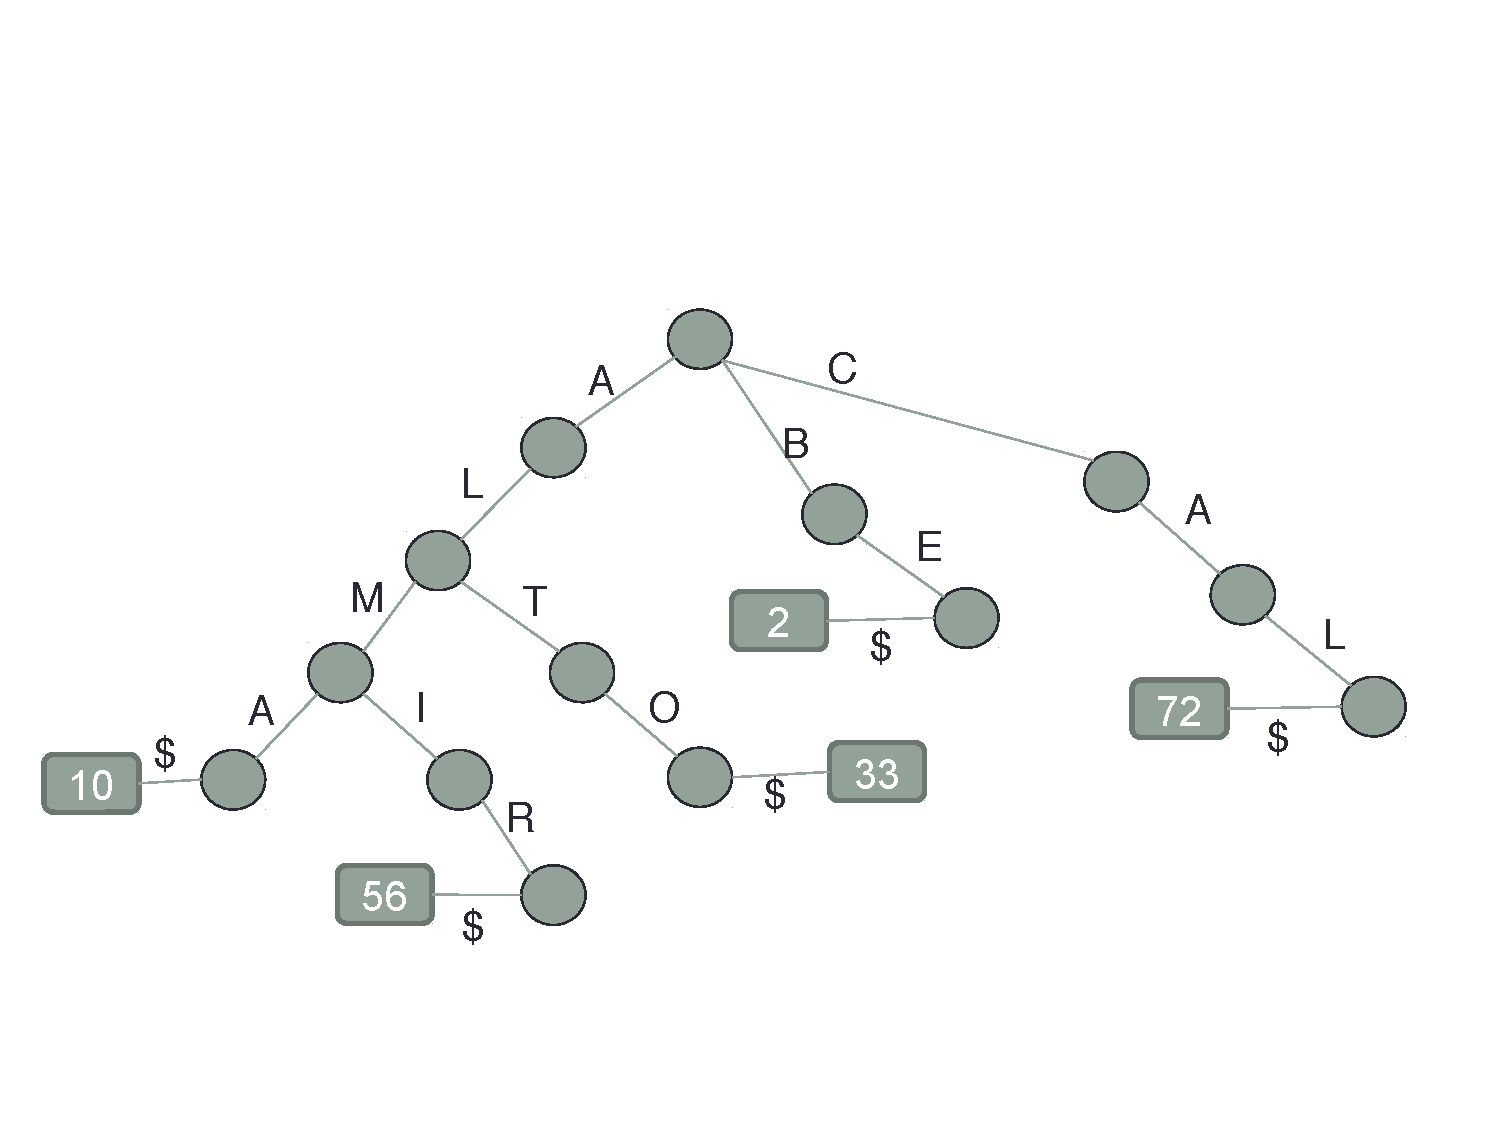
\includegraphics[width=0.7\textwidth]{aula05-trie1}
\caption{Exemplo de uma árvore Trie.}
\label{aula05:fig:trie1}
\end{figure}

\subsubsection{Chaves}

Uma chave é uma palavra sobre um alfabeto. 
Um símbolo é usado para indicar o término de uma chave. 
Esse símbolo deve ser um caractere que não faça parte do alfabeto, e garante
que uma chave não seja um prefixo de outra.
Dessa forma, os registros estarão nos nós folha da árvore.
%
\begin{description}
\item[Exemplo 1] tendo o alfabeto \{A, B, C, ..., Z\} e o símbolo
de término \$. Possíveis chaves: BOTA\$, CARRO\$, LEI\$.

\item[Exemplo 2] tendo o alfabeto \{0, 1, ..., 9\} e o símbolo de término \$.
Possíveis chaves: 134\$, 12978\$, 99777\$.
\end{description}
O caminho da raiz até um nó qualquer forma de um prefixo de uma chave indexada.

O formato das tries não depende da ordem em que as chaves são inseridas, depende
apenas dos valores das chaves.

\subsubsection{Estrutura de uma Trie}

A estrutura é composta de:
\begin{description}
\item[Nó raiz]  vazio e indexa nós que representem prefixos das chaves indexadas.
\item[Nós intermediários] prefixos de chaves de busca indexadas. Indexam outros nós
que aumentam o prefixo.
\item[Nós folha] chave completa e indexam as regiões de interesse. Ex.: offset da chave
de busca dentro de um arquivo de texto.
\end{description}

\subsubsection{Busca}

A busca começa pela raiz e pelo primeiro caractere.
Há dois cenários:
\begin{description}
\item[Cenário 1] o nó atual não é folha.
	\begin{enumerate}
	\item Se existe um filho que corresponda ao próximo caractere da chave.
		\begin{itemize}
		\item Avançar um caractere (passar a ignorá-lo a partir deste momento).
		\item Visitar o filho.
		\end{itemize}
	\item Se não existe esse filho.
		\begin{itemize}
		\item A chave não está indexada.
		\end{itemize}
	\end{enumerate}
\item[Cenário 2]  o nó atual é folha.
	\begin{enumerate}
	\item Esse nó de dados representa a resposta.
	\end{enumerate}
\end{description}

\subsubsection{Inserção}

Os passos da inserção são:
\begin{enumerate}
\item A palavra é buscada.
\item Se encontrar a palavra.
	\begin{enumerate}
	\item Adiciona-se um ponteiro no nó correspondente. O nó vira uma lista invertida contendo
	os offsets.
	\end{enumerate}
\item Caso contrário 
	\begin{enumerate}
	\item Localizar o último nó visitado.
	\item a partir desse nó, inserir o restante dos caracteres em novos nós.
	\end{enumerate}
\end{enumerate}

\subsubsection{Implementação}

Uma Trie pode ser implementada de duas formas diferentes:
\begin{itemize}
\item \textbf{R-Way} com nós de desvio e nós de informação. Os nós de desvio contem um filho para
cada símbolo do alfabeto mais um filho para o símbolo especial.

\item {\bf árvore TST (Ternary Search Tree)} ocupam menos espaço.
Cada nós possui um caractere e três ponteiros: próximo caractere (centro), 
caractere alternativo menor que o atual (esquerda), e caractere alternativo
maior que o atual (direita).
\end{itemize}

\subsubsection{Análise}

O custo em execução é $O(k m)$ para $k$ o tamanho do alfabeto e $m$ o tamanho da 
chave de busca.
O tempo de execução é independente do número de chaves, e a altura é igual ao comprimento da chave
mais longa.

O custo em espaço é $O(s)$ para $s$ a soma do tamanho de todas as chaves. 

\subsubsection{Trie compacta}

O espaço de uma Trie é reduzido por meio de compressão de nós redundantes, ou seja,
mesclando nós que possuem apenas um caminho possível.
A figura~\ref{aula05:fig:trie2} ilustra a versão compacta da  árvore Trie 
da figura~\ref{aula05:fig:trie1}.
%
\begin{figure}[ht]
\centering
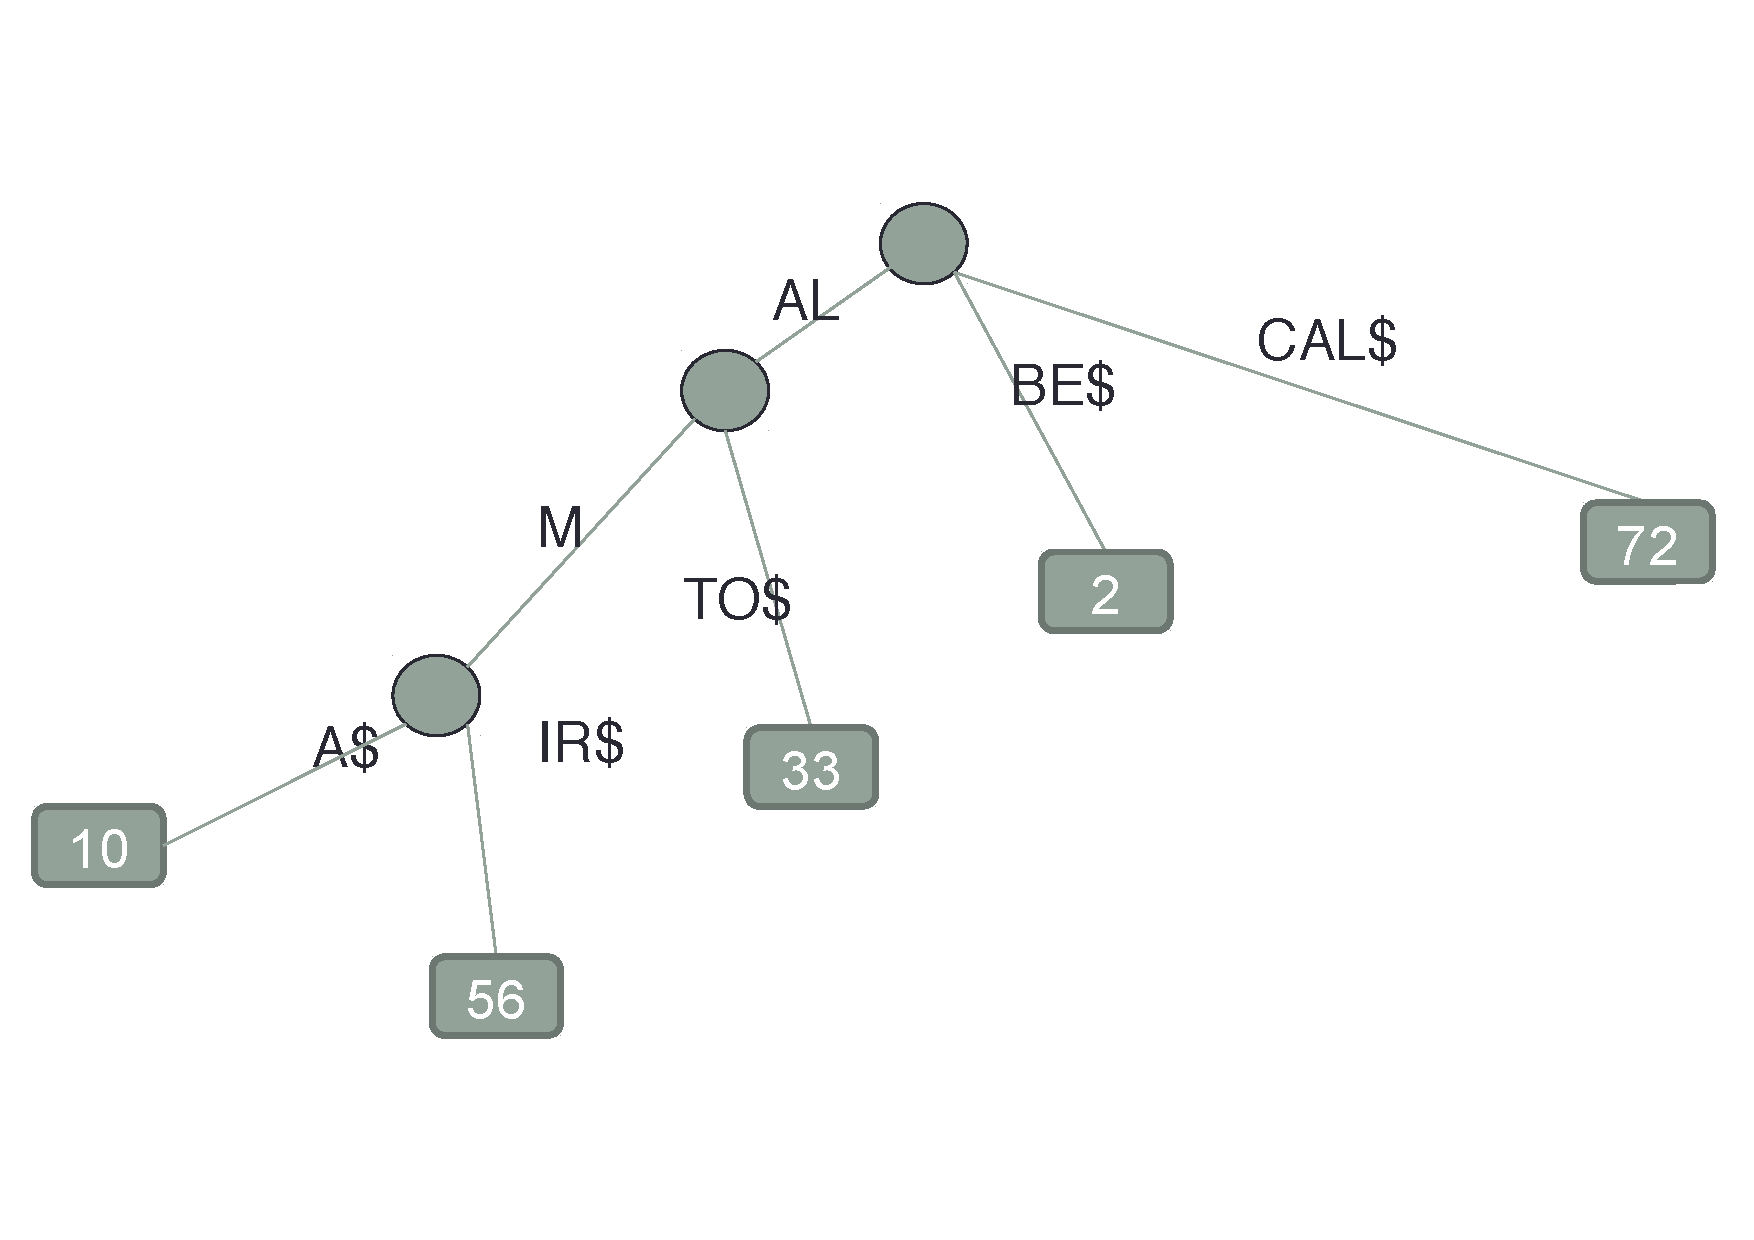
\includegraphics[width=0.6\textwidth]{aula05-trie2}
\caption{Exemplo de uma árvore Trie compacta.}
\label{aula05:fig:trie2}
\end{figure}

O custo em espaço de uma Trie compacta é $O(n)$ para $n$ o número de chaves, bem menor
que $O(s)$ da árvore não compacta. 
Todavia, o tempo de execução é o mesmo sendo $O(k m)$ para $k$ o tamanho do alfabeto e $m$
o tamanho da chave de busca.

\subsubsection{Trie binária}

Uma Trie binária é um tipo especial de Trie em que o alfabeto possui apenas 
apenas dois símbolos: \{0, 1\}.
Para compensar a ausência de símbolo especial, todas as cadeias de bits devem
ter o mesmo tamanho.
Caso alguma chave não tenha tamanho suficiente, basta preencher com 0s à
esquerda.

A figura~\ref{aula05:fig:trie3} ilustra um exemplo de árvore de árvore Trie binária
normal (esquerda) e compacta (direita) para os seguintes elementos:
\begin{itemize}
\item 0 - chave 000 valor 4.
\item 1 - chave 001 valor 22.
\item 4 - chave 100 valor 14.
\item 5 - chave 101 valor 39.
\end{itemize}
%
\begin{figure}[!htb]
\centering
  \begin{minipage}{0.4\textwidth}
	\centering
	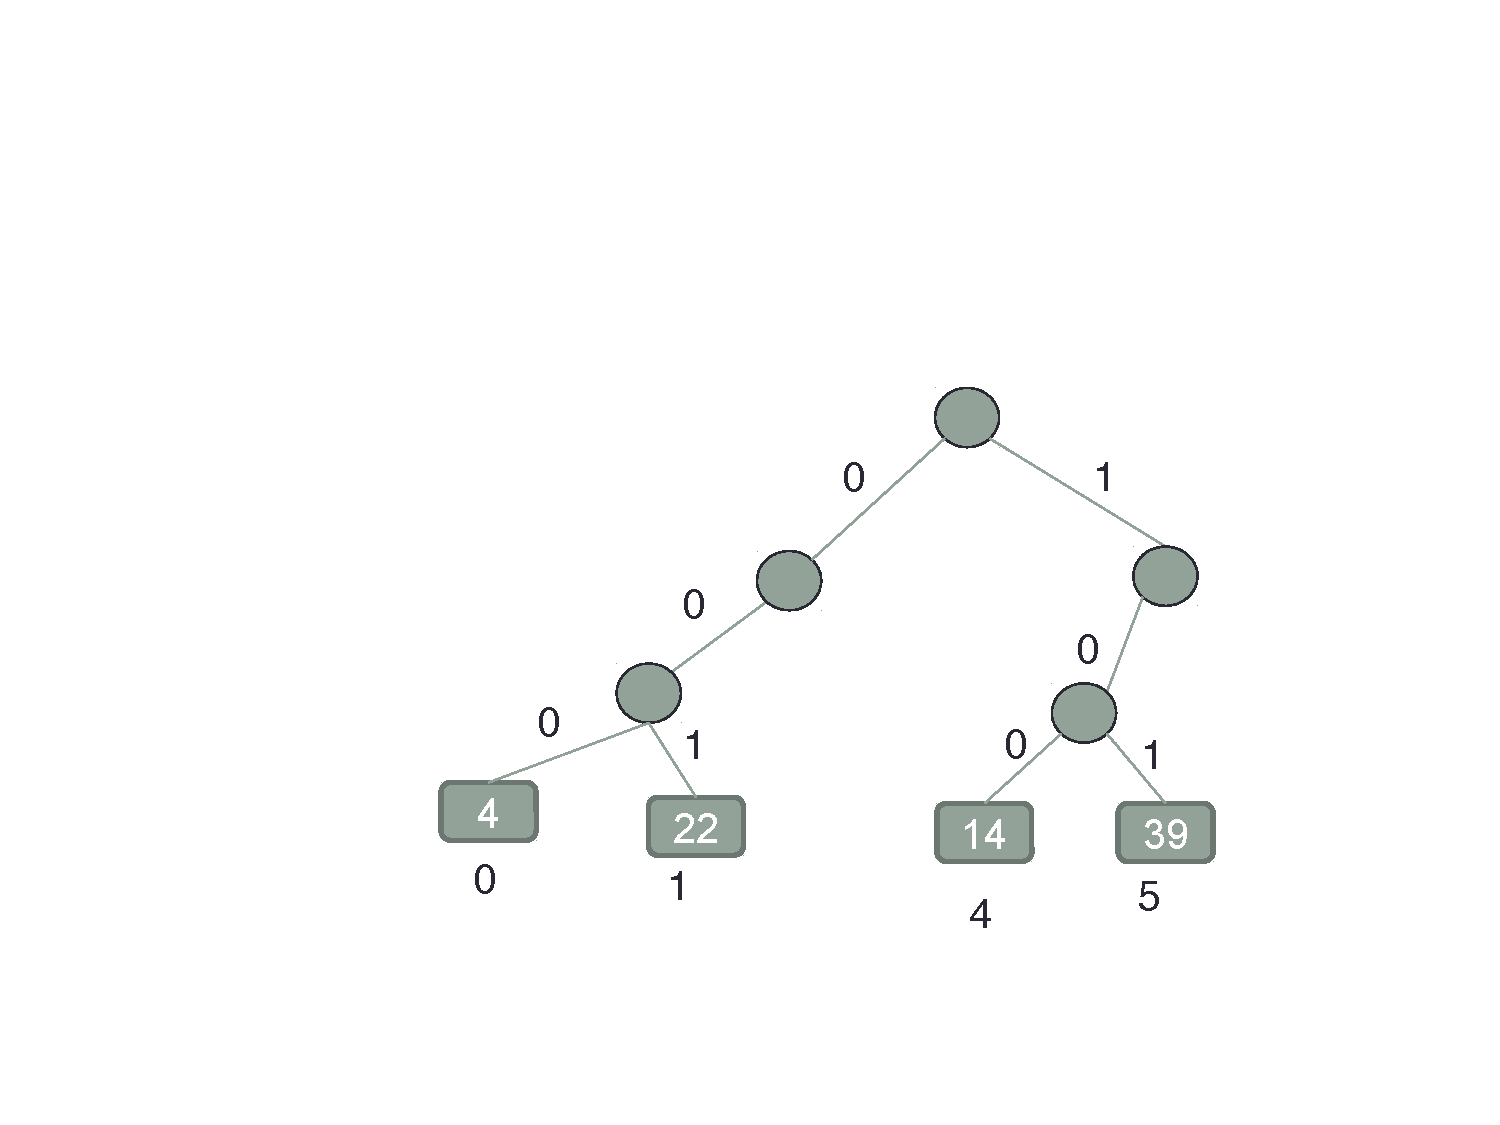
\includegraphics[width=\textwidth]{aula05-trie3}
  \end{minipage}
  %
  \vline
  %
  \begin{minipage}{0.4\textwidth}
	\centering
	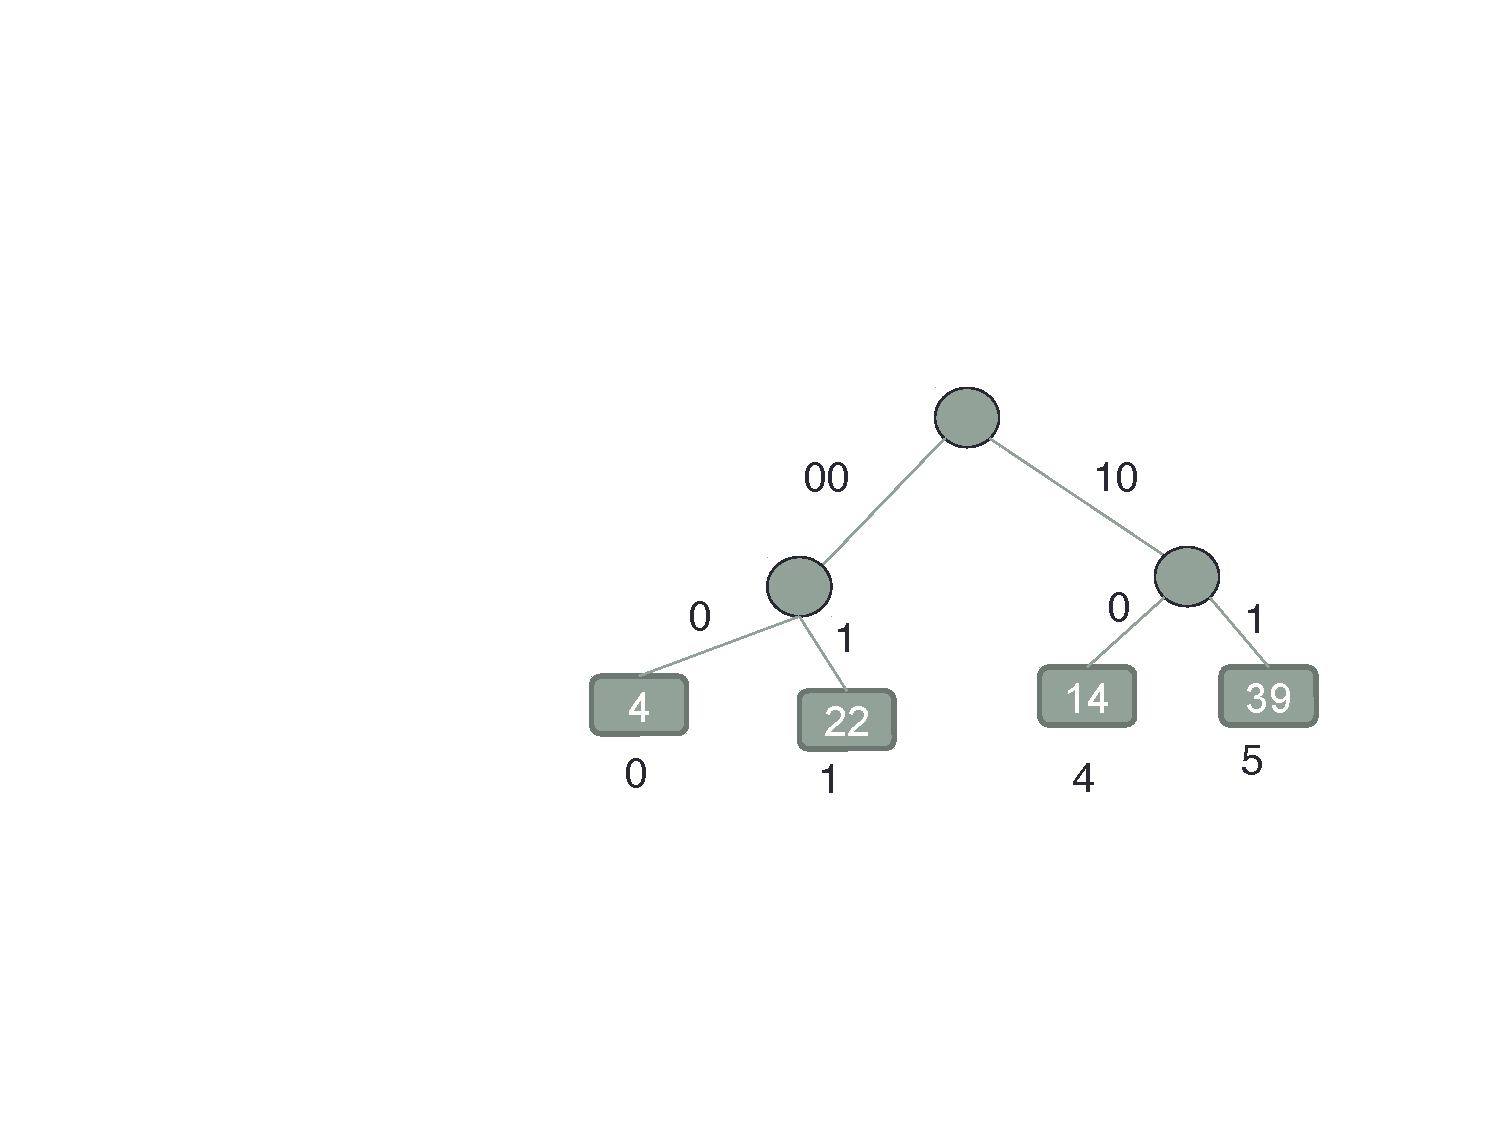
\includegraphics[width=\textwidth]{aula05-trie4}
  \end{minipage}
\caption{Exemplo de uma árvore Trie binária (esquerda) e binária compacta (direita).}
\label{aula05:fig:trie3}
\end{figure}

No pior caso, há $b$ comparações de bits, o que pode ser ineficiente quando as
chaves são grandes.  A versão compacta pode reduzir o custo, mas não o
suficiente.

%%%%%%%%%%%%%%%%%%%%%%%%%%%%%%%%%%%%%%%%%%%%%%%%%%%%%%%%%%%%%%%%%%%%%%%%%%%%%%%%
\subsection{Árvores Patricia}

Uma árvore Patricia, ou \emph{radix tree}, ou \emph{patricia trie}, vem do
acrônimo ``\emph{Practical Algorithm To Retrieve Information Coded In
Alphanumeric}'' e é uma árvore de busca compacta semelhante a uma Trie binária,
com alfabeto \{0, 1\}.
Entretanto, ela não usa um caractere especial para término (\$).
Todas as cadeias devem ter o mesmo tamanho.

Cada nó possui no máximo 2 filhos, e cada nó tem dois tipos: nós de desvio e nós de conteúdo.
Os nós de desvio possuem uma informação numérica que indica o bit da chave a testar.
A partir desse bit é decidido qual caminho da árvore a seguir.

A figura~\ref{aula05:fig:patricia1} mostra um exemplo de árvore Patricia e as
respectivas chaves.
Os valores dentro de cada nó indicam qual bit a ser testado no próximo desvio.
%
\begin{figure}[!htb]
\centering
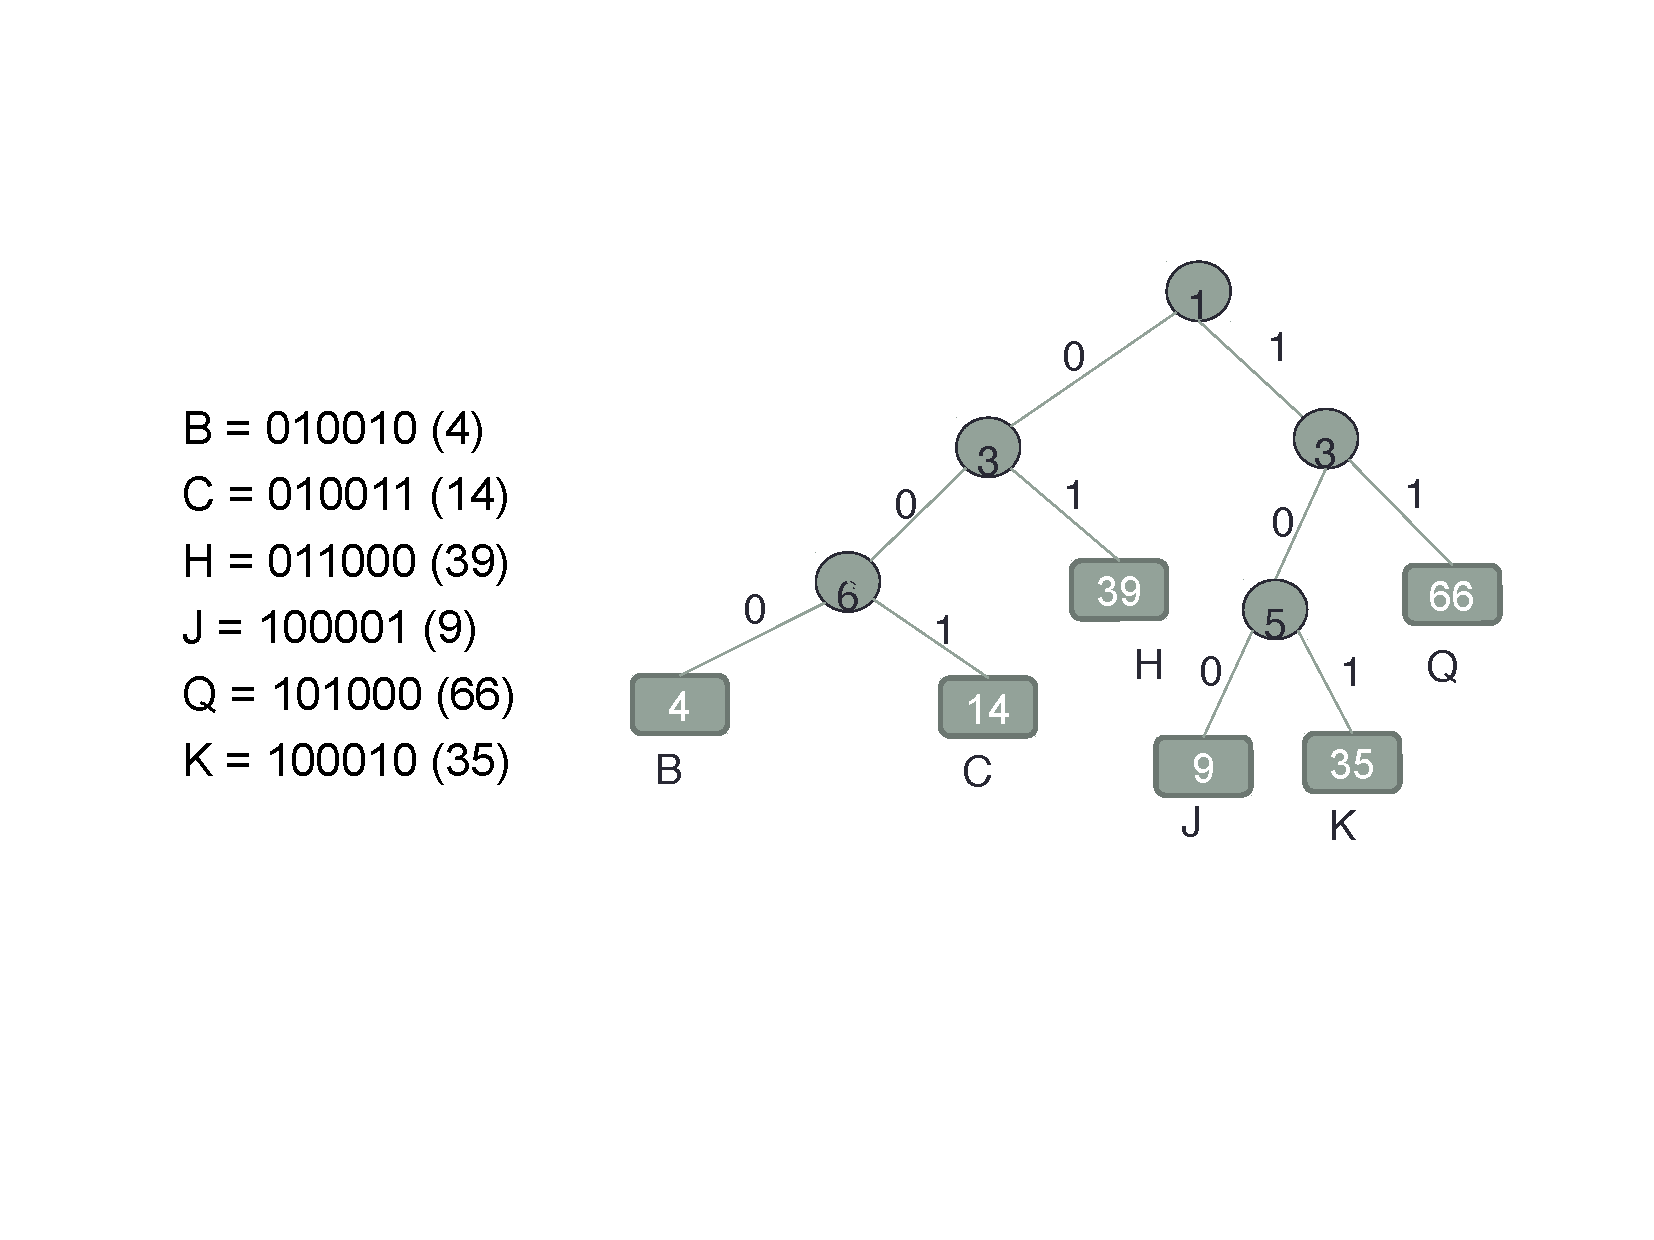
\includegraphics[width=0.6\textwidth]{aula05-patricia1}
\caption{Exemplo de uma árvore Patricia.}
\label{aula05:fig:patricia1}
\end{figure}

\subsubsection{Busca}

A busca começa pela raiz e pelo primeiro caractere (bit 0). 
Há dois cenários:
\begin{description}
\item[Cenário 1] o nó atual não é folha.
	\begin{enumerate}
	\item Verificar o dígito da chave de busca equivalente ao valor do nó.
	\item Se for 0, seguir a subárvore da esquerda.
	\item Caso contrário, seguir a subárvore da direita.
	\item Se não houver subárvore a seguir, a chave de busca não está indexada.
	\end{enumerate}

\item[Cenário 2] o nó atual é folha.
	\begin{enumerate}
	\item Deve-se verificar se o valor indexado realmente corresponde a chave de busca.
	\end{enumerate}
\end{description}

\subsubsection{Inserção}

Os passos da inserção em árvores Patricia são os seguintes:
\begin{enumerate}
\item A palavra (cadeia de bits) é buscada.
\item Se a árvore estiver vazia:
	\begin{enumerate}
	\item Cria-se uma estrutura inicial para indexar a palavra.
	\item Um nó raiz, com valor igual a 1, e um nó filho (a esquerda ou direita), indexando
		a palavra.
	\end{enumerate}
\item Se a busca parar em um nó anterior a um nó folha.
	\begin{enumerate}
	\item Significa que o nó só possui um único filho.
	\item Cria-se o outro filho, que indexará a palavra inserida.
	\end{enumerate}

\item Se a busca parar em um nó folha.
	\begin{enumerate}
	\item o conteúdo indexado é comparado com a palavra a ser inserida.
	\item se for igual, é adicionada uma entrada no nó folha para a palavra indexada.
	\item Se for diferente.
		\begin{enumerate}
		\item é preciso descobrir o nó da árvore a ser atualizado.
		\item para isso, é verificada a posição $P$ do primeiro bit onde ocorre a
			diferença.
		\item Se o bit for {\bf maior} que a última posição utilizada, deve-se adicionar um nó aqui.
		\item Se o bit for {\bf menor}  que a última posição utilizada, deve-ser subir na árvore
			para encontrar o local adequado. 
		\end{enumerate}
	\end{enumerate}

\item Para o caso de subida na árvore.
	\begin{enumerate}
	\item Sobe-se na árvore até encontrar o nó $X$, o nó mais baixo cujo
		valor seja maior que a posição $P$.
	\item Nesse ponto é inserido um novo nó, tendo como filhos:
		\begin{enumerate}
		\item O nó $X$.
		\item Um novo nó para indexar a nova palavra.
		\end{enumerate}
	\item Os ponteiros e valores dos nós criados/remanejados são atualizados.
	\end{enumerate}
	
\end{enumerate}

%%%%%%%%%%%%%%%%%%%%%%%%%%%%%%%%%%%%%%%%%%%%%%%%%%%%%%%%%%%%%%%%%%%%%%%%%%%%%%%%
\subsection{Aplicações de Tries e Patricia}

As Tries de caracteres podem ser aplicadas em:
\begin{itemize}
\item Verificadores de ortografia.
\item Motores de busca - nós folhas guardam páginas que possuem a palavra indexada.
\end{itemize}

As Tries binárias são usadas na compressão de dados, como na Codificação de Huffman.

As árvores Patricia podem ser usadas na indexação de chaves longas.

%%%%%%%%%%%%%%%%%%%%%%%%%%%%%%%%%%%%%%%%%%%%%%%%%%%%%%%%%%%%%%%%%%%%%%%%%%%%%%%
\section{Exercícios}
%%%%%%%%%%%%%%%%%%%%%%%%%%%%%%%%%%%%%%%%%%%%%%%%%%%%%%%%%%%%%%%%%%%%%%%%%%%%%%%

\begin{enumerate}
\item Descreva os passos da busca binária e os custos para o melhor caso, caso médio
e pior caso.

\item Qual é a principal característica de uma árvore binária de pesquisa ?

\item Descreva a árvore binária de busca criada a partir dos seguintes elementos:
$5, 8, 3, 6, 7, 1, 9, 4$.

\item A partir da árvore do exercício anterior, descreva a árvore binária de busca
resultante da remoção dos seguintes elementos: $4, 5$.

\item Desenhe a árvore AVL resultante da inserção dos números: 
$9, 8, 7, 6, 5, 4, 3, 2, 1$.

\item Escreva o algoritmo para imprimir o \textsc{menor} elemento de uma árvore de busca binária.
\item Escreva o algoritmo para imprimir o \textsc{maior} elemento de uma árvore de busca binária.

\item Escreva dois algoritmos que recebem uma árvore AVL como entrada: para
imprimir todos os elementos em ordem crescente e decrescente.

\item Considere a seguinte lista de valores: $[0, 9, 10, 3, 8, 4, 5, 1]$. 
	\begin{enumerate}
	\item Construa  uma árvore binária de busca não balanceada.
	\item Construa  uma árvore AVL.
	\end{enumerate}

\item Para uma árvore binária de busca:
	\begin{enumerate}
	\item Descreva um algoritmo {\bf não recursivo} que faz um percurso em-ordem.
	\item Descreva algoritmos recursivos para percursos pré-ordem e pós-ordem.
	\item Descreva algoritmos recursivos para buscar o elemento mínimo
		(\lstinline{ArvoreMinimo}) e elemento máximo
		(\lstinline{ArvoreMaximo}).
	\end{enumerate}

\item  Supondo que temos números de $1$ a $1000$ em uma árvore binária de busca,
e queremos buscar o número $363$. Quais das sequencias abaixo {\bf não} 
poderiam ser sequencias de nós percorridos nessa busca ?
	\begin{enumerate}
	\item $2,252,401,398,330,344,397,363$.
	\item $924, 220, 911, 244, 898, 258, 362, 363$.
	\item $925, 202, 911, 240, 912, 245, 363$.
	\item $2,399,387,219,266,382,381,278,363$.
	\item $935, 278, 347, 621, 299, 392, 358, 363$.
	\end{enumerate}

\item Desenhe uma árvore rubro-negra com chaves ${1, 2, ..., 15}$.
Adicione os nós folhas com \textsc{NIL} e faça coloração dos nós de forma
que o $bh(x)$ (\emph{black-height} ou altura-preto) da árvore seja 2, 3 e 4.

\item Mostre a árvore rubro-negra resultante depois de inserir sucessivamente
os nós ${41, 38, 31, 12, 19, 8}$ em uma árvore vazia.

\item Agora, baseado no exercício anterior,  mostre a árvore rubro-negra
resultante da remoção dos nós ${8, 12, 19, 31, 38, 41}$ sucessivamente.

\item Para as palavras chave da seguinte frase ``Marcos Lima marcou o marco'', e
	considerando o alfabeto \{a, b, ..., z\}, crie:
	\begin{enumerate}
	\item uma Trie compacta em formato de árvore.
	\item uma Trie normal, em formato R-Way.
	\item uma Trie normal, em formato TST.
	\end{enumerate}
Obs: artigos não precisma ser indexados.

\item Dadas as seguintes cadeias de bits: 00101 valor 5, 11000 valor 15, 01010 valor 34,
10101 valor 23, 11111 valor 12, 01110 valor 77. Crie:
	\begin{enumerate}
	\item uma Trie binária compacta.
	\item uma árvore Patricia.
	\end{enumerate}

\end{enumerate}
